%**************************************************
%TEMPLATE TAKEN FROM: 
%https://seanbone.ch/latex-template-exam-summary/
%**************************************************

% Use extarticle for the smaller font size:
% https://tex.stackexchange.com/questions/5339/how-to-specify-font-size-less-than-10pt-or-more-than-12pt
\documentclass[a3paper, 8pt]{extarticle}

\usepackage[document]{ragged2e}

% Multi-column layout
\usepackage{multicol} \setlength\columnsep{9pt}
\usepackage{graphicx}
\graphicspath{ {./images/} }

% Manually set page margins
\usepackage[margin=0.5cm, bmargin=0.8cm, landscape]{geometry}

\usepackage{centernot}
%\usepackage[T1]{fontenc}
%\usepackage{lmodern}

\usepackage{xcolor}
\usepackage{soul}

\newcommand{\notiff}{%
  \mathrel{{\ooalign{\hidewidth$\not\phantom{"}$\hidewidth\cr$\iff$}}}}

% TO DO
% MORE HEAD SPACES FOR THEOREMS
% Replace graphics from slides with grpahics form Lecture notes
% Margins of pictures
% Name theorems correctly
% Less space after Definition
% Manually set margins on lists
\usepackage{enumitem}
% Change list margins - https://tex.stackexchange.com/questions/10684/vertical-space-in-lists
\setlist{leftmargin = 4mm, nosep, topsep=0pt}
% \setlist{noitemsep} to leave space around whole list
%create new list type
\newlist{mylist}{enumerate}{4}

\setlist[itemize]{topsep=0pt, nosep, parsep=0pt, leftmargin=3mm}


%Defining a Definition for proofs and stuf


\usepackage{amsmath}
\usepackage{mathtools}
\usepackage{amssymb}
\usepackage{graphicx}
\usepackage[english]{babel}
\usepackage{blindtext}
\usepackage{amsthm}
\usepackage{gensymb}
\usepackage{parskip}
\usepackage{titlesec}
\usepackage{xcolor}
\usepackage{comment}
\usepackage[dvipsnames]{xcolor}

\usepackage[parfill]{parskip}


\titleformat{\section}
[hang]
{\RaggedRight \fontsize{13}{13} \sc}
{\thesection}
{5pt}
{}
[\hrule]

\titleformat{\subsection}
[hang]
{\RaggedRight \fontsize{10}{10} \sc}
{\thesubsection}
{4pt}
{}
[\hrule]

\titleformat{\subsubsection}
[hang]
{\RaggedRight}
{\thesubsubsection}
{4 pt}
{}
[\hrule]

%\titleformat{\paragraph}
%[hang]
%{\RaggedRight \underline}
%{}
%}
%{}
%[\pr]



%\titlespacing{\paragraph}{}{3pt}{4pt}

\titlespacing{\subsection}{}{6pt}{4pt}

\titlespacing{\subsubsection}{0pt}{8pt}{4pt}

\titlespacing{\section}{}{10pt}{6pt}

\usepackage{amsmath}

\usepackage{amsthm}
\newtheorem{theorem}{Theorem}[section]

\newtheorem*{theorem*}{Theorem}

\newtheorem{corollary}{Corollary}[theorem]

\newtheorem{proposition}{Proposition}[section]

\newtheorem*{corollary*}{Corollary}

\newtheorem{lemma}[theorem]{Lemma}

\newtheorem*{definition}{Definition}

\newtheorem*{remark}{Remark}



\title{Compressed exam summary}
\author{Paul Gruenenwald}

\usepackage{amsmath} % Required for the \numberwithin command
\makeatletter % enable access to internal commands with @ symbol
\@addtoreset{equation}{section} % Reset equation counter at start of every section
\makeatother % disable access to internal commands with @ symbol
\renewcommand{\theequation}{\arabic{equation}} % Remove section number from equation number


\begin{document}
% Make formulas more compact
%Better alternative to sections
% 3-column layout

%\fontsize{6pt}{6pt}\selectfont
%\tiny
%\scriptsize
%\renewcommand{\familydefault}{\rmdefault}

\setlength{\abovedisplayskip}{6pt}
\setlength{\belowdisplayskip}{6pt}
\setlength{\abovedisplayshortskip}{5pt}
\setlength{\belowdisplayshortskip}{5pt}
\setlength{\columnseprule}{0.2pt}


\RaggedRight



\begin{multicols*}{5}

\section{Regression Assumptions}
$$Y_i=\beta_0+\beta_1X_{1i}+\beta_2X_{2i}+\epsilon_i$$

\begin{enumerate}
    \item The model is linear in parameters and \textbf{correctly specifed}
    \item There is no exact multicollinearity between the independent variables in the regression equation.
    \item The \textbf{conditional distribution of the error term has zero expectation} $E (\epsilon_i | X_{1i} , X_{2i} ) = 0$.
    \item The error term is homoskedastic (i.e., constant variance).
    \item The values of the error term have independent distributions.
    \item[\Rightarrow] These assumptions are often violated!
\end{enumerate}

\section{OVB}
OVB occurs when a relevant variable that affects the dependent variable is left out of the model, leading to biased and inefficient parameter estimates. 

\begin{tabular}{l l}
   \hl{Estimate:}   & \hl{$Y_i=\beta_0+\beta_1X_{1i}+\epsilon_i$} \\
    \hl{True model:} & \hl{$Y_i=\alpha_0+\alpha_1X_{1i}+\alpha_2X_{2i}+\epsilon_i$}
\end{tabular}

No OVB $\Leftrightarrow \ \alpha_2=0  \ \land \  Corr(X_{2i}, X_{1i})= 0$
$$\hat{\beta}_1=\frac{\Sigma_{i=1}^N (X_{1i}- \Bar{X}_1)(Y_i-\Bar{Y})}{\Sigma_{i=1}^N (X_{1i}- \Bar{X}_1)^2}= \frac{Cov(X_1,Y_1)}{Var(X_1)}$$

$\hat{\beta}_1$ will be unbiased if $E(\hat{\beta}_1 | X) = \beta_1$
$$E(\hat{\beta}_1 | X) = \alpha_1 + \alpha_2 \rho + 0$$

\hl{$\rho$ is the coefficient from a regression of $X_2$ on $X_1$: \\ $X_2 = \beta_0 + \rho X_1 + \epsilon$}

\subsection{\hl{Estimating bias}}


\hl{Downward bias $\equiv$ negative }  $ \Leftrightarrow \alpha_2 \rho$ negative $\Leftrightarrow$  Estimate is smaller than the true parameter


\hl{Upward bias $\equiv$ positive}  $ \Leftrightarrow \alpha_2 \rho$ positive $\Leftrightarrow$  Estimate is larger than the true parameter

understating $\Rightarrow$ the estimated absolute effect is smaller than the absolute true parameter

overstating $\Rightarrow$ the estimated absolute effect is larger than the absolute true parameter

\section{Binary Dependent Variable}
\subsection{Linear Probability Model}

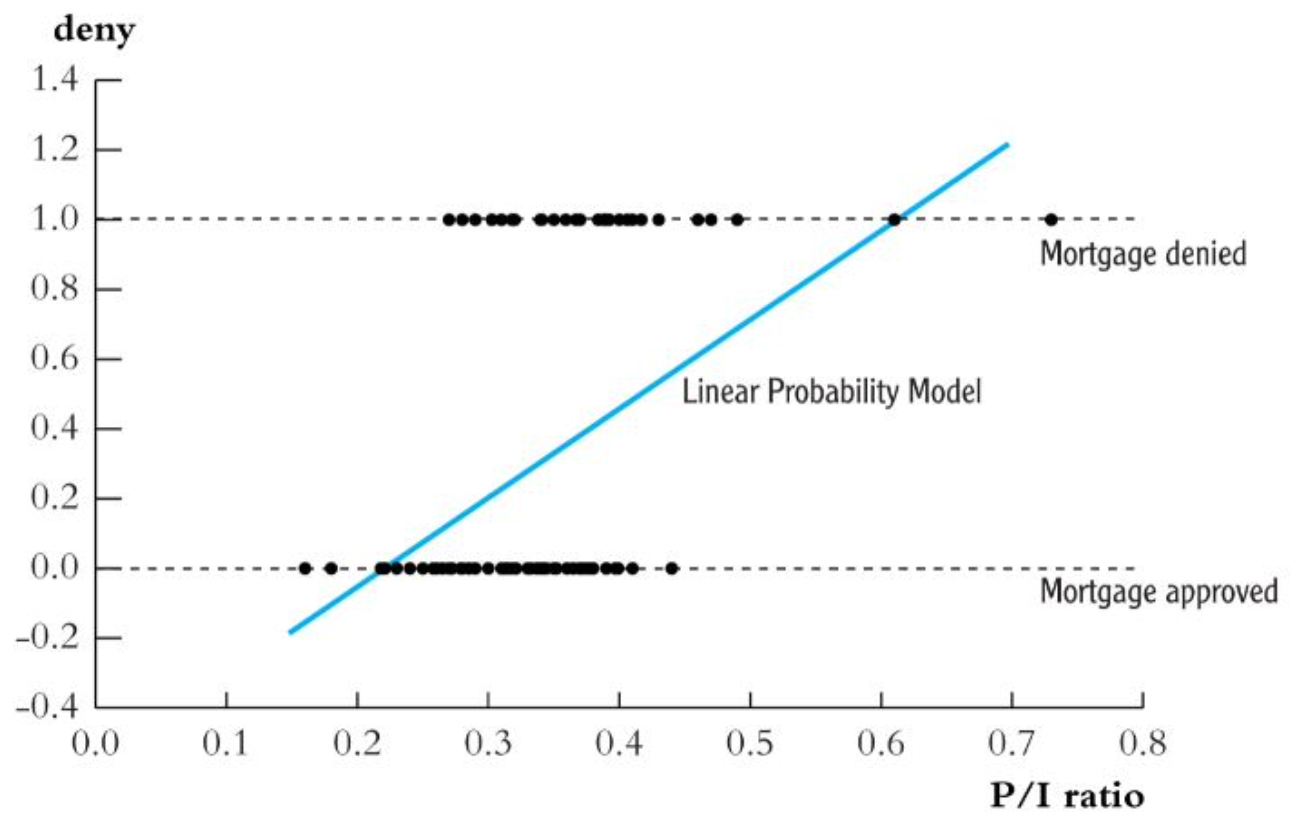
\includegraphics[width =  \columnwidth]{Screen Shot 2023-03-12 at 15.30.59.png}

In the linear probability model, the predicted value of $Y$ is interpreted as the predicted probability that $Y=1$, and $\beta_1$ is the change in that predicted probability for a unit change in $X$. When Y is binary, the linear regression model.

$$Y_i = \beta_0 + \beta_1 X_i + u_i$$

Least squares assumption: $E(u_i | X_i)=0$, so when $Y$ is binary: %$E(Y_i | X_i) = E(\beta_0 + \beta_1 X_i + u_i | X_i) $
$$Pr(Y_i=1 | X)= \beta_0 + \beta_1 X_i$$
$$\beta_1=\frac{Pr(Y=1|X=x+ \Delta x)-Pr(Y=1 | X=x)}{\Delta x}$$

\subsection{Index Models}

Index models restrict the response to be between 0 and 1: $Pr(Y|X)=F(\beta_0+\beta_1X)$ where $0 \leq F(.) \leq 1$

Any function $F(.)$ that maps a real number to a real number between 0 and 1 works.

\subsection{Probit Regression}

The problem with the linear probability model is that it models the probability of Y =1 as being linear:

We need a function that transforms the linear input into an "S-curve"...

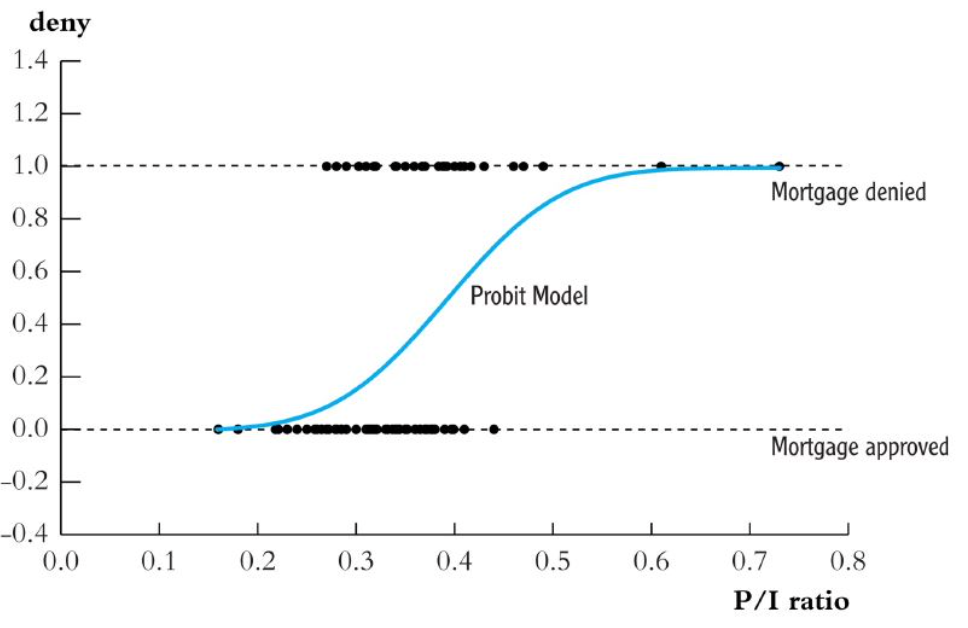
\includegraphics[width= \columnwidth]{Screen Shot 2023-05-29 at 11.20.59.png}

$$Pr(Y=1|X)=F(\beta_0+\beta_1 \cdot X) = \phi (\beta_0 + \beta_1 X)$$

$\phi$ is the cumulative normal distribution function


\subsection{Logit Regression}

$$Pr(Y|X)=F(\beta_0+\beta_1 X) = \frac{exp(\beta_0 + \beta_1 X)}{1+exp(\beta_0 + \beta_1 X)}= \Lambda(\beta_0 + \beta_1 X) $$

 $\Lambda(\beta_0 + \beta_1 X)$ is the cumulative distribution function (CDF) of the standard logistic distribution

\subsection{Latent Variable Interpretation of Logit/Probit}
In the latent variable model, the continuous variable Y* represents an unobserved latent variable, while Y represents the binary outcome variable derived from Y* using a threshold crossing rule.

\paragraph{threshold crossing rule} refers to the process of converting the continuous latent variable Y* into a binary outcome variable Y based on a predetermined threshold.


\subsection{Measures of Fit}
\paragraph{Fraction correctly predicted}







\subsection{Maximum-Likelihood-Estimator (MLE)}
Non-linear equations are estimated using MLE.

It finds parameters of a joint probability distribution that make it most likely that, if we would draw the data again, we would get observations similar to those that we have.

Let's say you go to a NRA rally and ask 10 NRA supporters if they want teachers to be given guns. 8 say yes, i.e. in your sample a fraction of 0.8 are pro-gun.

 which parameter p would make it most likely that you observe the answers that you got? $\Rightarrow p=0.8$

 \subsubsection{Deriving the MLE}
 In general, you come up with a formula for the probability that you draw exactly the observations that you have, and then you maximize this expression.

As draws are independent (i.i.d.), the probability that they happen all at the same time is simply the product of the individual probabilities.
$$P(Y_1=y_1, Y_2=y_2 ...)=P(Y_1=y_1)\cdot P(Y_2=y_2)...$$
To simplify calculations you then take logs (product → sum!)
$$ln(P(Y1 = y1))+ln(P(Y2 = y2))$$

Then maximize (i.e., FOC=0), and say hi to your MLE.

\subsubsection{Special Case: probit MLE with no X}

$$Y= \begin{cases} 1 \ \text{with probability $p$}\\
0 \ \text{with probability $1-p$}\end{cases}$$
(Bernoulli distribution)
$$Pr(Y_1=y_1, Y_2=y_2, ..., Y_n=y_n)= p^{\Sigma_{i=1}^n y_i} (1-p) ^{n-\Sigma_{i=1}^n y_i}$$



\section{Matching}
Matching aims to address the issue of confounding variables in observational studies. It aims to create comparable treatment and control groups by matching participants who are similar in terms of their observed characteristics or covariates.

The basic idea behind matching is to identify individuals in the treatment group who closely resemble individuals in the control group in terms of their observed covariates. By doing so, the distribution of confounding variables is balanced between the two groups, reducing the potential bias caused by these variables.

\subsection{Assumptions}

\paragraph{Conditional independence assumption} It states that, conditional on the observed covariates (matching variables), the assignment to the treatment or control group is independent of potential outcomes.

\paragraph{Common support} The matching variables must have overlapping ranges of values between the treatment and control groups. This ensures that there are individuals in the control group who have similar values of the matching variables as those in the treatment group.

\subsection{Identify matching variables}


\subsection{Determine the matching algorithm}

\subsubsection{Bandwidth}The researcher does have to define how close is “close.”

Small bandwidth means that your estimate of Y0(x) is probably pretty accurate, but imprecise because you are averaging over a small number of obs.

Large bandwidth means that your estimate of Y0(x) may be less accurate, but more precise because you are averaging over a larger number of obs.

\subsubsection{k-nearest neighbor matching}
Larger k means smaller variance, but may mean greater bias.

One way to estimate $\hat{Y}_0(x)$ is to find the point closest to the point x, $x_{min}(x)$.

$$\hat{Y}_0(x)=Y_0(x_{min}(x))$$

$C^0 (x_i)$ are the $k$ observations with $D=0$ and $X$ closest to $x_i$

$w_{ij}=1 / k$: equal weights

\subsubsection{Caliper Matching}
Choose a distance, or caliper $\delta$, such that all comparison obs. whose distance is within $\delta$ of the treatment obs. are averaged to form $Y_0(x)$.



$C^0 (x_i)= \{j:|x_i -  x_j| < \delta \}$; all $k $ observations within a window of size \delta.

$w_{ij}=1 / k$: equal weights

\subsubsection{Kernel based matching}
Idea: use more observations, but give weight in proportion to the ‘closeness’ of observables.

\begin{center}
    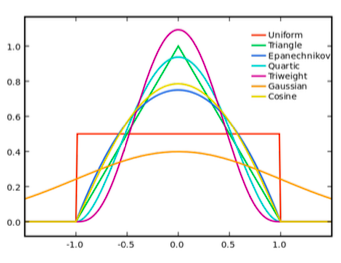
\includegraphics[width = 0.7 \columnwidth]{Screen Shot 2023-05-29 at 15.19.14.png}
\end{center}

$C^0 (x_i)= \{j:D_j = 0 \}$; use all untreated observations.

$w_{ij}=f(x_i - x_k)


\subsubsection{\hl{Propensity Score Matching}}

\paragraph{Curse of dimensionality} We can quickly run out of data if we have to match on multiple continuous variables. Same is true if we have to match on lots of discrete variables.

Thus we create a single variable upon which we do the matching: The propensity score $p(x)$ measures the probability of being in the treatment group given the observed covariates or characteristics of individuals. It is estimated through a statistical model, typically logistic regression, that predicts the likelihood of treatment assignment based on the covariates.

The propensity score is used as a balancing score in matching analysis to create comparison groups that are similar in observed characteristics. By matching individuals with similar propensity scores, the goal is to achieve balance between the treated and control groups, reducing the influence of confounding variables.

Once you have the propensity score, you still have to choose a method by which to match comparison observations to treatment observations. You can use one of the approaches discussed before. (k-nearest neighbor-, caliper-, kernel matching).

\subsubsection{\hl{Estimating the propensity score with Cell estimators}} With discrete data you can form cells that represent all combinations of every possible value of X.

To create the propensity score, you count the number of treated observations and the number of total observations for each value of X. So for each X = x, estimate p(x) by

$$p(x)=\frac{n_{x, D=1}}{n_x}$$

\subsubsection{\hl{Estimating the propensity score with OLS, Logit or Probit}}With many variables X (especially if continuous) you suffer from the course of dimensionality when trying to estimate p(x) with the cell estimator

Often people simply assume linearity and use OLS/Probit/Logit to estimate: $D = \gamma X + u$

Side note: alternatively, use machine learning methods - they are intended for prediction!

\texttt{probit D x1 x2 x3 x4\\
predict px}

\subsection{Assess Balance}
balance refers to the similarity or comparability of the treated and control groups in terms of their observed characteristics or covariates.

Ideally, you want to check that the distribution of Xs is the same for the treated and untreated groups, which implies checking for similarity of means, variances, as well as higher moments.


\subsection{Estimate treatment effects}

\subsubsection{Cell Estimator}
The cell estimator is the simplest possible matching estimator, but it can only be used with discrete data.

Divide data into "cells" defined by all possible values of the covariates.

For each value of X = x, i.e., each cell, compare the mean outcomes of treated and untreated observations to calculate the treatment effect at X = x.

\begin{center}
    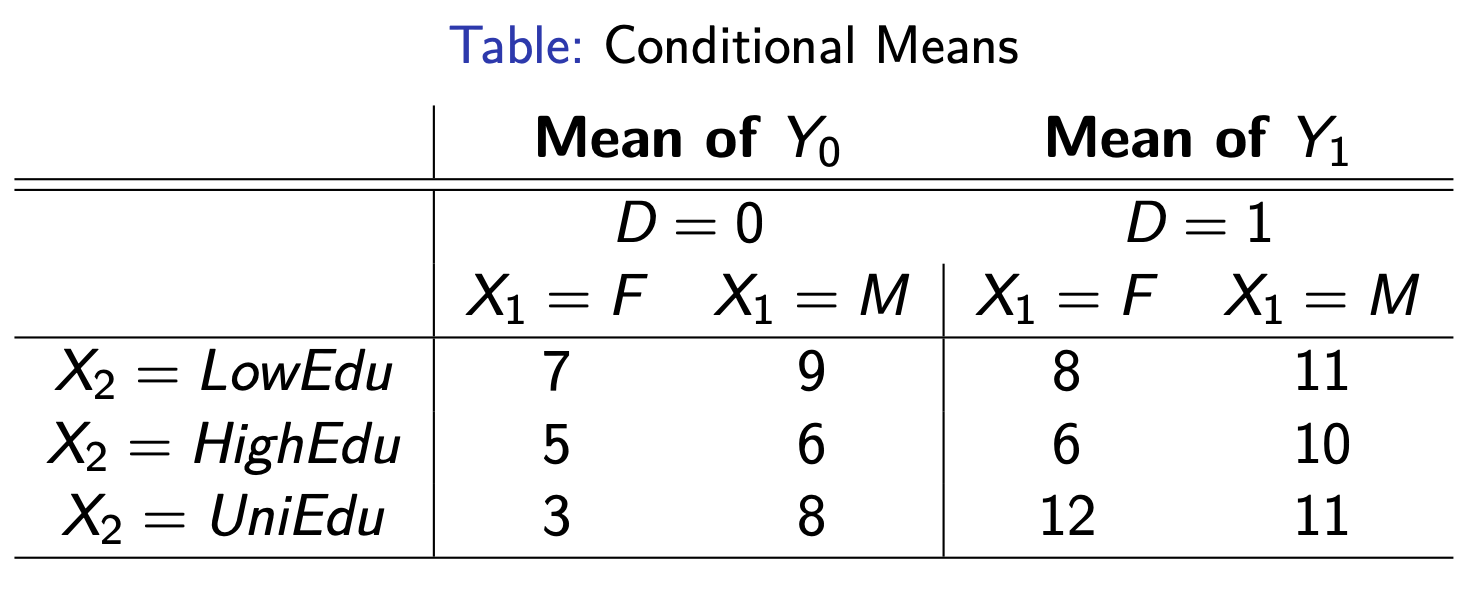
\includegraphics[width = 0.8 \columnwidth]{Screen Shot 2023-03-23 at 18.14.12.png}

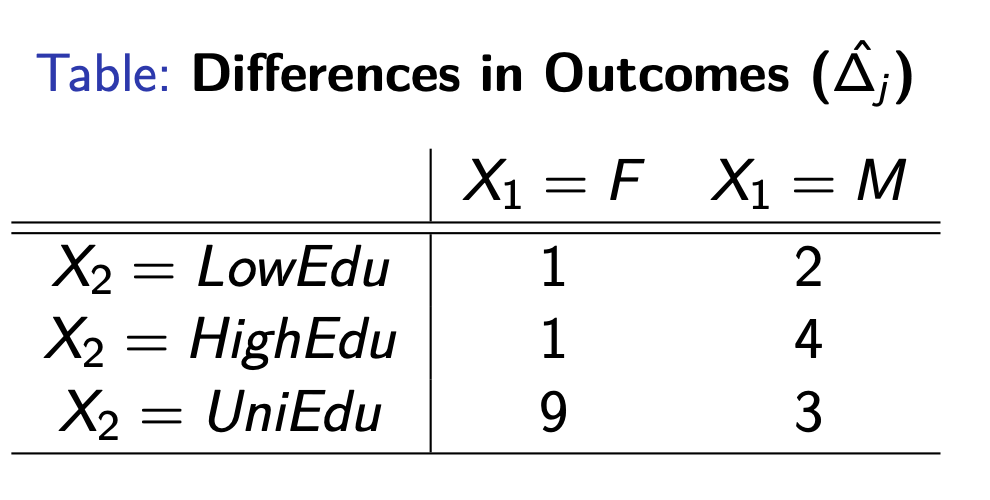
\includegraphics[width = 0.55 \columnwidth]{Screen Shot 2023-03-23 at 19.20.17.png}
\end{center}

\paragraph{Average Treatment Effect (ATE)}
To calculate this we need the frequency of each cell

\begin{center}
    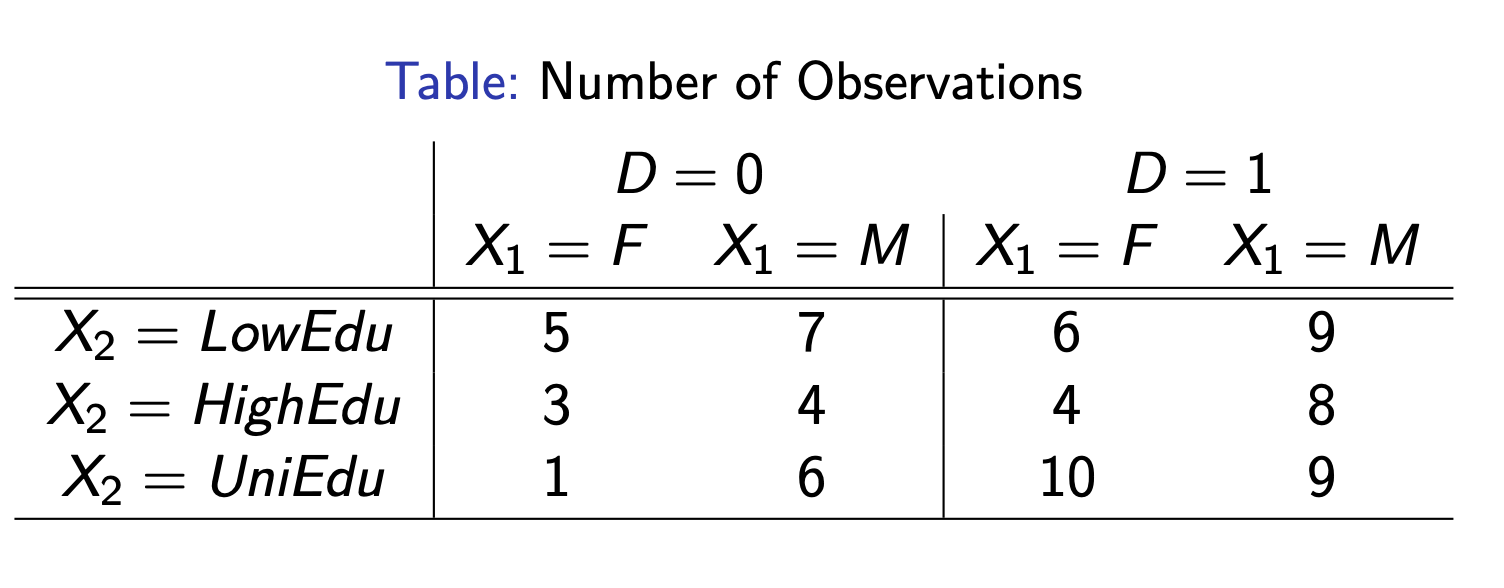
\includegraphics[width = 0.9 \columnwidth]{Screen Shot 2023-03-23 at 19.23.44.png}
\end{center}

Get a weighted average of the differences in outcomes according to the frequency of each cell.

In calculating these estimates, we did not have to specify a functional form for the regression function.

This is the most non-parametric estimator possible. We are comparing simple means of different groups.

\subsubsection{General Matching Estimator}
$$\hat{Y}_0(x_i)=\Sigma_{j\in C^0(x_i)} w_{ij}Y_0(x_j)$$

\begin{tabular}{l l}
  $C^0(x_i)$   & the set of untreated neighbors of treated $i$\\
   $w_{ij}$  & $\in [0,1]$ with $\Sigma_{j \in C^0(x_i)}w_{ij}=1$
\end{tabular}

Suppose X is continuous and we observe a treated observation with X = x.

We want to estimate the counterfactual outcome Y0 at the point X = x. Denote this by $\hat{Y}_0(x)$.

Problem: we do not have any untreated people with X = x.

Solution: take observations with X “close” to x and average their Y0.


\subsubsection{Inverse Propensity Score Weighting}
is a method used to estimate treatment effects in observational studies by accounting for the propensity score, which represents the probability of treatment assignment given the observed covariates. 

IPSW assigns weights to individuals based on their propensity scores, adjusting for potential confounding variables.

This is done to give more weight to individuals who are less likely to receive the treatment and less weight to individuals who are more likely to receive the treatment. In essence, it amplifies the contribution of the control group members who are similar to the treated group members, but received different treatments.

The cost of this is that some observations carry a lot more weight than others (especially an issue if they are outliers).

\begin{tabular}{l l}
    Untreated group & \hl{$w_j=\frac{1}{(1-p(x_j))}$} \\
    Treated group & \hl{$w_j=\frac{1}{p(x_j)}$}
\end{tabular}

This gives a larger weight to people who are unusual, given their treatment status.

To get the estimate of the treatment effect you can run the following \textbf{weighted} regression
$$y=\beta_0 + \beta_1 D + u$$
\paragraph{Weighted regression}
 is a statistical technique used to perform regression analysis while assigning different weights to individual data points.

\section{Panel Data}

$$(X_{it},Y_{it}), i=1, ...,n, t=1, ..., T$$

A double subscript distinguishes entities (states) and time periods (years) i = entity (state), n = number of entities,
so i = 1,...,n

t = time period (year), T = number of time periods so t =1,...,T

Another term for panel data is longitudinal data

balanced panel: no missing observations, that is, all variables are observed for all entities (states) and all time periods (years)

With panel data we can control for factors that: Vary across entities but do not vary over time
Are unobserved or unmeasured - and therefore cannot be included in the regression using multiple regression

Here's the key idea:
If an omitted variable does not change over time, then any changes in Y over time cannot be caused by the omitted variable.

$$FatalityRate_{it}=\beta_0+\beta_1BeerTax_{it}+\beta_2Z_i+u_{it}$$


\subsection{Fixed Effects}
$$Y_{it}=\beta_0+\beta_1X_{it}+\beta_2Z_i+u_{it}$$
\subsubsection{Fixed Effects regression model}
letting $\alpha_i=\beta_0+\beta_2Z_i$ we get the model


\begin{equation}
    Y_{it}=\alpha_i+\beta_1X_{it}+u_{it}
\end{equation}
the $\alpha_i$ doesn't change over time, it is the intercept for a given state. The intercept is unique but the slope is the same in all the states.


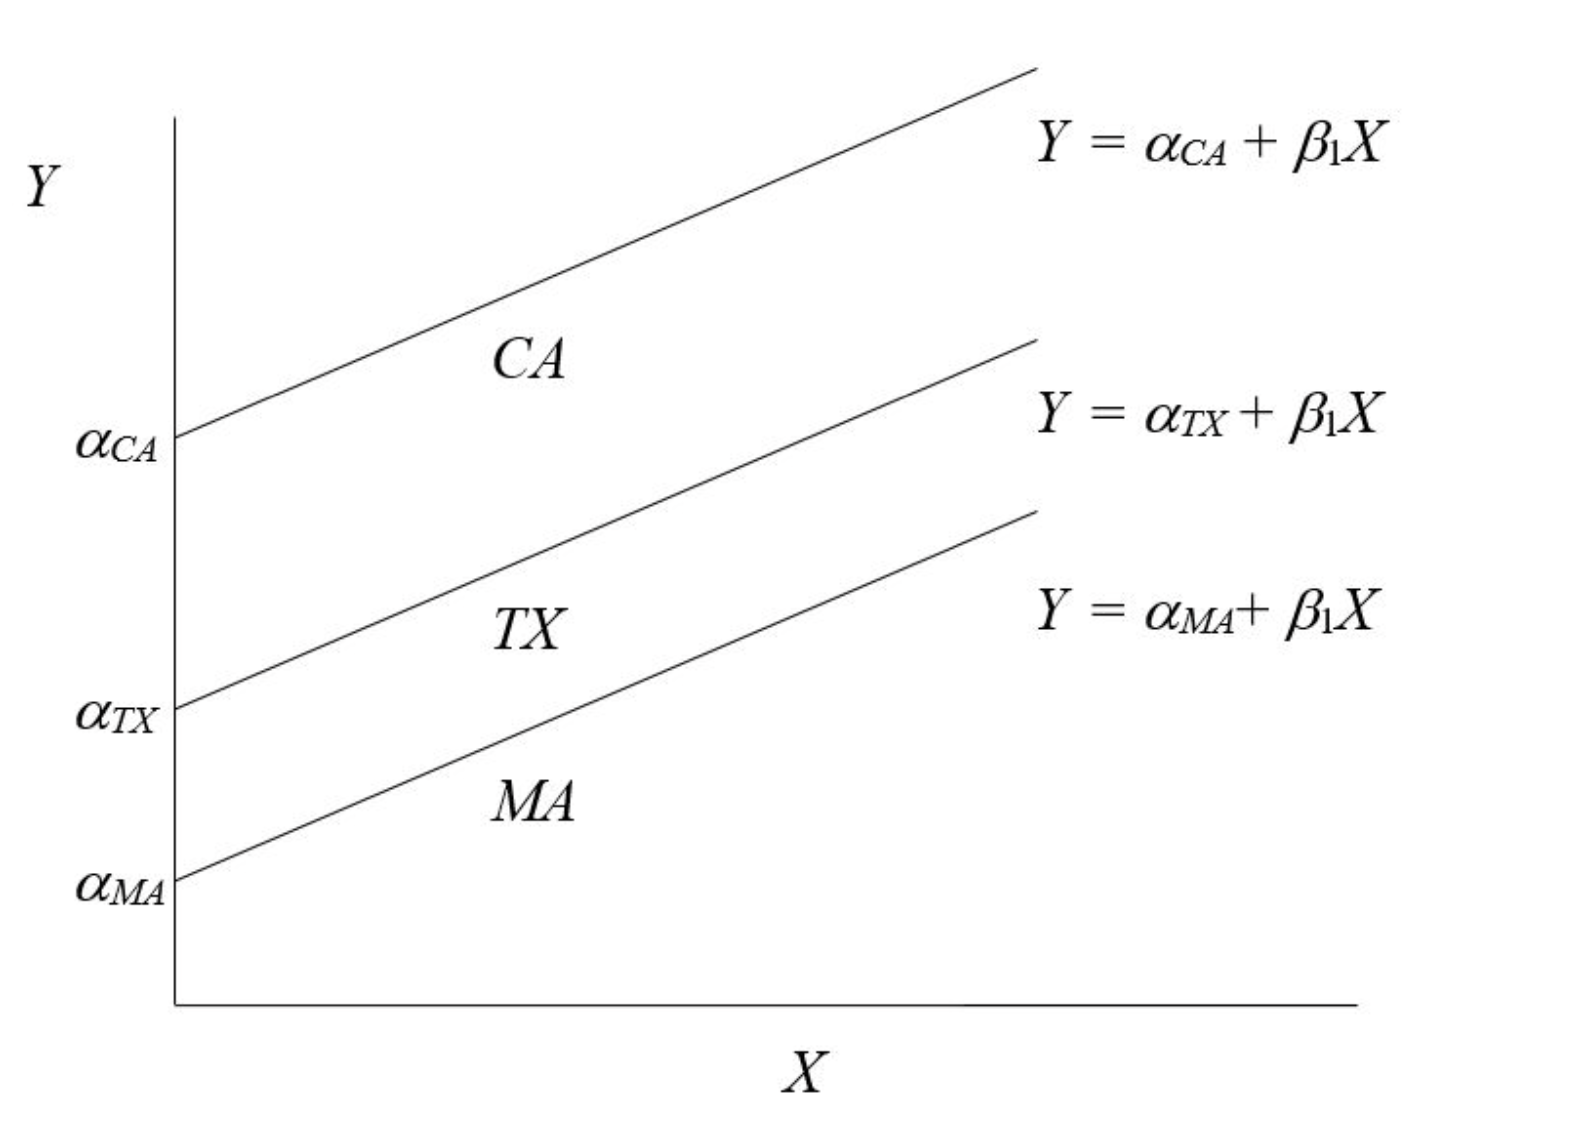
\includegraphics[width = \columnwidth]{Screen Shot 2023-03-18 at 21.28.01.png}

\subsubsection{n-1 binary regressor form}
$$Y_{it}=\beta_0+\gamma_{2}D2_i+...+\gamma_{n}Dn_i+\beta_1X_{it}+u_{it}$$
$D2_i= 1$ if state is CA, $= 0$ otherwise \\
$Dn_i= 1$ if state is TX, $= 0$ otherwise

\subsubsection{Estimation Methods}
\paragraph{Entity-demeaned OLS regression}
The entity averages satisfy:
$$\underbrace{\frac{1}{T}\Sigma_{t=1}^T Y_{it}}_{\Bar{Y}_i}=\alpha_1 + \beta_1 \underbrace{\frac{1}{T}\Sigma_{t=1}^T X_{it}}_{\Bar{X}_i} +\underbrace{\frac{1}{T}\Sigma_{t=1}^T u_{it}}_{\Bar{u}_i}}$$

\begin{tabular}{l l}
    $\alpha_1$ & average Y for all entities \\
    $\beta_1$ &  average effect of X on Y \\
     & 
\end{tabular}

the equation is stating that the average value of Y for each entity can be explained by the intercept term, the average value of X, and the average unobserved factors. 

By demeaning the data, we are able to remove the entity-specific fixed effects, allowing us to focus on the average relationships between variables while controlling for entity-specific heterogeneity.

Deviation from entity averages:
$$Y_{it}-\frac{1}{T}\Sigma_{t=1}^T Y_{it}= \beta_1(X_{it}-\frac{1}{T}\Sigma_{t=1}^T X_{it})+(u_{it}-\frac{1}{T}\Sigma_{t=1}^T u_{it})$$
or $$\Tilde{Y}_{it}=\beta_1 \Tilde{X}_{it}+ \Tilde{u}_{it}$$
$\Tilde{X}_{it}$ and $\Tilde{Y}_{it}$ are "entity-demeaned" data.

For i=1 and t = 1982, $\Tilde{Y}$ is the difference between the fatality rate in Alabama in 1982, and its average value in Alabama averaged over all 7 years.

\begin{equation}
    \Tilde{Y}_{it}=\beta_1 \Tilde{X}_{it}+ \Tilde{u}_{it}
\end{equation}

Where $\Tilde{Y}_{it}=Y_{it}-\frac{1}{T}\Sigma_{t=1}^T Y_{it}$ etc.

\begin{enumerate}
    \item Construct entity-demeaned variables $\Tilde{Y}_{it}$ $\Tilde{X}_{it}$
    \item Estimate the model by regressing $\Tilde{Y}_{it}$ on $\Tilde{X}_{it}$ using OLS
    \item Standard errors need to be computed in a way that accounts for the panel nature of the data set (more later)
\end{enumerate}
\paragraph{Changes specifcation} without an intercept (only works for T = 2)



\subsubsection{Assumptions Fixed Effects}
Assumptions under which the fixed effects regressor is asymptotically normally distributed for large enough N

Least squares regression assumptions to panel data
\begin{enumerate}
    \item Linearity
    \item Strict exogeneity: The error term is uncorrelated with all the explanatory variables, including the time-invariant fixed effects.
    \item No perfect multicollinearity
    \item Homeoscedasticity: The variance of the error term is constant across all observations
    \item Balanced panels
    \item Adequate number of states
    \item ...
\end{enumerate}

\subsubsection{Regression Assumptions Fixed Effects}


\begin{enumerate}
    \item Error term $u_{it}$ has mean zero, given the state fixed effect and the entire history of the $X$'s for that state.
    $$E(u_{it} | X_{i1}, ... X_{iT}, \alpha_1)=0$$
    This means ther are no omitted  \textbf{lagged effects}
    and no \textbf{feedback from $u$ to future $X$}. Whether a state has a particularly high fatality rate this year doesn't subsequently affect whether it increases the beer tax.
    \item variables for one state are distributed identically (but independently) of the variables for another state.

    This is satisfied if entities (states, individuals) are randomly sampled from their population by simple random sampling, then data for those entities are collected over time.

    \item Large outliers are unlikely: (Xit, uit) have finite fourth moments.
\end{enumerate}

\subsubsection{Standard Errors Fixed Effects}


\paragraph{Clustered standard errors}
a type of heteroskedasticity and autocorrelation-consistent (HAC) standard errors

The term clustered arises because the standard errors allow the regression errors to have an arbitrary correlation within a cluster (or grouping) but assume that the regression errors are uncorrelated across clusters.

In the context of panel data, a cluster is a state

Clustered standard errors allow for heteroskedasticity and autocorrelation within a state (entity) but treat the errors as uncorrelated across states.


They are consistent with the second fixed effect assumption. They are valid whether or not there is heteroskedasicity and/or autocorrelation.


If the number of states is large, inference can proceed using the usual large-sample normal critical values for t-stats and F-stats (usually you need >40 clusters).



Notice that assumption #2 allows $X_{it}$ to be correlated over time within a state (entity)

It is common, for example, what happens in one year tends to be correlated with what happens in the next year (beer tax is correlated over time in a state)

\paragraph{autocorrelated} correlated with itself at different dates

$u_{it}$ might also be autocorrelated $\to$
 we need to make sure the standard error calculation allows for autocorrelation.

Intuition: if uit is correlated over time, you don't have as much information (as much random variation) as you would have if $u_{it}$ were uncorrelated.


In addition, we still need to consider that the errors might be heteroskedastic.

\paragraph{heteroskedastic} variance of errrors is not constant with X

\subsection{Time and Entity Fixed Effects}



\subsection{Fixed Effects and Multicollinearity}
\paragraph{Excluded constant} and include all time and entity fixed effects, you need to \hl{exclude either one entity fixed effect or one time fixed effect}

\paragraph{Included constant} you would have to \hl{exclude one entity fixed effect and one time fixed effect}.



\section{Instrumental Variables (IVs)}

Instrumental Variable (IV) estimation is a statistical technique used to address OVB by providing a strategy to deal with endogeneity in regression models.

It relies on the use of instrumental variables, which are variables that are correlated with the endogenous independent variable but are unrelated to the error term. These instruments serve as a source of exogenous variation, mimicking the random assignment of treatments in a randomized controlled trial (RCT).

The key idea behind IV estimation is to use the instruments to "instrument" or replace the endogenous variable in the regression model.


$$Y_i =\beta_0+\beta_1 X_i+u_i$$

IV regression breaks X into two parts: \begin{enumerate}
    \item a part that might be correlated with $u$
    \item a part that is not
\end{enumerate}
→ By isolating part 2, it is possible to get a consistent estimate of $\beta_1$

\subsection{Threats to internal validity}

\begin{enumerate}
    \item OVB that affects both $Y$ and $X$ but that is unobserved
    \item Simulatenous causality bias / reverse causality ($X$ causes $Y$, but $Y$ also causes $X$)
    \item Measurement error bias ($X$ is measured with error
\end{enumerate}
IV regression can solve all these problems

\paragraph{Internal validity} the ability to establish a causal relationship between the endogeneous variable of interest (e.g. PC ownerhsip) on the outcome variable (e.g. GPA score)



\paragraph{Endogeneity}
refers to a situation in which a variable in a statistical model is correlated with the error term, or the unobserved factors that affect the dependent variable. This correlation can occur when there are omitted variables, measurement errors, or simultaneous causality, which can lead to biased or inconsistent estimates.

When a variable is correlated with the error term, it means that there is a systematic relationship between this variable and the unobserved factors that affect the dependent variable. 

\subsubsection{Intention to Treat variable}
If you observe whether the subject actually receives treatment ($D$), and if you know whether the individual was initially assigned to a treatment group ($Z$) (and if initial assignment was random), then you can estimate the causal effect using initial assignment as an instrument for actual treatment. In this case, $Z$ is also called the intention-to-treat variable.

\subsection{Valid IVs}


\begin{enumerate}
    \item \hl{Instrument exogeneity}:
    The instrument should be uncorrelated with the error term in the model. This means that the IV(s) should not be correlated with any unobserved factors that affect the outcome variable, besides through its effect on the endogenous variable of interest. The instrumental variable(s) should have no direct effect on the outcome variable.
    \item \hl{Instrument relevance}: The instrument must be correlated with the endogenous variable of interest (in this case, PC ownership) and be a significant predictor of it.
    \item Validity: The instrument should not only satisfy the above properties but must also be a valid instrument for the specific causal question being asked.
\end{enumerate}

\subsection{Two-stage least squares (TSLS)}
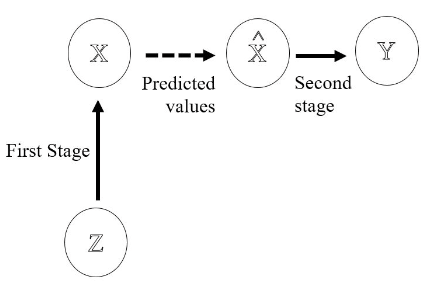
\includegraphics[width = 0.9 \columnwidth]{Screen Shot 2023-03-31 at 16.46.45.png}

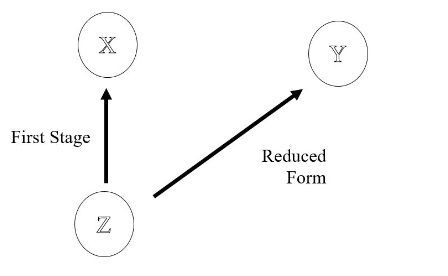
\includegraphics[width = 0.9 \columnwidth]{Screen Shot 2023-03-31 at 16.46.54.png}


\paragraph{First Stage} relates $X$ to $Z$:
\begin{equation}
    X_i=\pi_0+\pi_1Z_i+v_i
\end{equation}

decomposes $X$ into a problematic part that is correlated with $u$ and another part that is uncorrelated with the $u$

The component $$\pi_0+\pi_1Z_i$$
 is the part of $X$ that can be predicted by $Z$.

We don't know $\pi_0$ $\pi_1$ so in the first stage, we estimate equation $(1)$ by OLS and get the predicted values of $X_i$ :
$$\hat{X}_i=\hat{\pi}_0+\hat{\pi}_1Z_i+ v_i$$
\paragraph{Reduced form} relates $Y$ directly to $Z$
$$Y_i=\gamma_0+\gamma_1Z_i+w_i$$



\paragraph{Second stage} uses the problem-free component to estimate $\beta_1$

Regress $Y_i$ on $\hat{X}_i$ (including an intercept); the
coefficient on $\hat{X}_i$ is the TSLS estimator, $\hat{\beta}_{TSLS}$.

$$Y_i= \beta_0 + \beta_1 \hat{X}_i+ u_i $$

A unit change in $Z_i$ causes a change in $X_i$ of $\pi_1$ and a change in $Y_i$ of
$\gamma_1$.

The reduced form is the causal impact of $Z$ on $Y$. The first stage tells us, if the entire effect runs through $X$, how much of a change in $X$ it took to cause the effect on $Y$.


To get the effect on Y in terms of X-units, you have to rescale the reduced form effect by the first stage effect.

\hl{TSLS-Estimator:}

$$\hat{\beta}=\frac{\gamma_1}{\pi_1}$$

\textbf{In other words, the IV estimator is the reduced form divided by
the first stage.}


\paragraph{Another way to see this:}
\begin{align*}
    Y_i &=\beta_0+\beta_1X_i+u_i\\
cov(Y_i,Z_i)&=cov(\beta_0+\beta_1X_i+u_i,Z_i)\\
&=cov(\beta_0, Z_i) + cov(\beta_1X_i, Z_i) +cov(u_i,Z_i)\\
&=0 + cov(\beta_1X_i,Z_i)+0\\
&=\beta_1 cov(X_i, Z_i)
\end{align*}

Thus: $$\beta_1=\frac{cov(Y_i,Z_i)}{cov(X_i,Z_i)}$$

Note that: $$\text{Reduced form:  }\gamma_1=\frac{cov(Z,Y)}{var(Z)}$$
$$\text{First stage: }\pi_1=\frac{cov(Z,X)}{var(Z)}$$

where $cov(u_i, Z_i)=0$ by instrument exogeneity and $cov(\beta_0, Z_i)=0$ because the covariance between a constant and a random variable is always zero.

\hl{Important note on standard errors}:
The OLS standard errors from the second stage regression are not right they do not take into account the estimation in the first stage ($\hat{X}$ is estimated).
Instead, \hl{use a single specialized command that computes the TSLS estimator and the correct SEs}.


\subsection{Checking for weak instruments}

\subsubsection{First-stage F-statistic}.
Rule-of-thumb: If the first stage F-statistic is less than 10, then the set of instruments is weak.

If you have many instruments, some are probably weaker than others and it's a good idea to drop the weaker ones

\subsubsection{Overidentification test}

\paragraph{Identification} In general, a parameter is said to be identified if we can obtain an unbiased estimator of that parameter from our data.


In IV regression, whether the coefficients are identified depends on the relation between the \hl{number of instruments ($m$)} and the \hl{number of endogenous regressors ($k$)}

Intuitively, if there are fewer instruments than endogenous regressors, we can't estimate $\beta_1, ..., \beta_k$

\paragraph{Overidentification} 
If there are more instruments than endogenous regressors, and if effects are not heterogenous.

Overidentification can help address the potential issue of treatment effect heterogeneity. 

If there are more instruments than endogenous regressors, and if effects are not heterogenous (no LATE) it is possible to test partially for instrument exogeneity.

Instrument exogeneity refers to the condition that the instruments used in instrumental variable (IV) analysis are uncorrelated with the error term in the regression model. If the instruments are exogenous, they satisfy the necessary condition for identification and provide consistent estimates of the causal effect.


\begin{tabular}{l l}
    \hl{exactly identified} & \hl{if $m = k$} \\
    \hl{overidentified} & \hl{if $m > k$} \\
    \hl{underitentified} & \hl{if $m < k$} \\
\end{tabular} 

\subsubsection{Testing overidentification restrictions}
assesses the validity of the instruments employed in an IV model and examines whether the assumptions underlying the instrumental variable approach hold.

\paragraph{J-Test}
When researchers have more instruments than the minimum required to identify the parameters of interest. This can be used to check the validity of the instruments and ensure that they are not correlated with the error term in the equation. Using the J-Test.

Suppose there are two valid instruments: Z1i, Z2i Then you could compute two separate TSLS estimates.

Intuitively, if these 2 TSLS estimates are very different from each other, then something must be wrong: one or the other (or both) of the instruments must be invalid.

This can only be done if #Z's > #X's (overidentified) and if effects are homogenous (strong assumption!).


\subsubsection{Left-Hand Side-Test of exclusion restriction (LHS)}



\paragraph{Exclusion restriction} It states that the instruments used in the analysis should affect the endogenous explanatory variable only through their impact on the outcome variable and not through any direct influence on the outcome variable.

Is another way to assess validity of Instruments:

Put some of the control variables on the left-hand side of the regression equation (obviously not those controls that are included for the exogeneity of the instrument for those we already know that there is a correlation with the instrument, and it's "part of the story").

Run:
$$W_{1,i} =\beta_0 +\beta_1 Z_i + \beta_2 W_{2i} + ... + \beta_r W_{ri} +u_i$$



\hl{If $\beta_1$ is signifficant, it shows that the exclusion restriction fails.}



\subsection{Validity}

\subsection{Internal validity}
Is the instrument relevant and exogenous?

\subsection{External validity}
Can the outcome be generalized?

\subsection{Measurement errors}

\subsubsection{Attenuation Bias}
With increased variance of the error term (e.g. due to more measurement error) estimated coefficients are biased towards zero.


\section{Experiments \& Quasi-Experiments}

\paragraph{experiment} is designed and implemented consciously by human researchers. An experiment randomly assigns subjects to treatment and control groups (think of clinical drug trials).

\paragraph{quasi-experiment} or natural experiment has a source of randomization that is "as if" randomly assigned, but this variation was not the result of an explicit randomized treatment and control design.

\paragraph{average treatment effect} is the population mean value of all the individual treatment effects.

\paragraph{potential outcome} is the outcome under a potential treatment or potential non-treatment.

An individual's causal effect can never be observed because you can give the subject the treatment, or not but not both!
You only observe one of the potential outcomes!
The other unobserved potential outcome is also called the \textbf{counterfactual} (outcome).

\subsection{Regression}

We observe $(Y_i, D_i)$, where $Y_i$ is the observed outcome.
\begin{align*}
    Y_i&=Y_i(1)D_i + Y_i(0)(1-D_i)\\
    &=\beta_{0i} + \underbrace{\beta_{1i}}_{Y_i (1) - Y_i (0)} D_i + u_i
\end{align*}
\begin{tabular}{l l}
    $i$ & subject $i$ \\
    $D_i=1$ & subject treated \\
    $D_i=0$ & subject not treated \\
    $Y_i(0)$ & potential outcome for subject $i$ if untreated \\
    $Y_i(1)$ & potential outcome for subject $i$ if untreated \\
    $\beta_{1i}$ & individual causal effect \\
    $Y_i (0), D_i =1$ & unobserved counterfactl potential outcome
\end{tabular}

\subsection{Randomization based on Covariates}
 Randomization in which the probability of assignment to the treatment group depends on one or more observable variables $W$ is called randomization based on covariates.

 \subsubsection{Example}

 To estimate the causal effect of mandatory versus optional homework in an econometrics course. In that experiment, economics majors were assigned to the treatment group with higher probability than nonmajors. 
 
 But if majors tend to do better in the course than nonmajors anyway, then \hl{there is omitted variable bias because being in the treatment group is correlated with the omitted variable, being a major.}

 \hl{Because $X_i$ is randomly assigned given $W_i$,
 this omitted variable bias can be eliminated by using the additional control variable $W_i$} (dummy for major/nonmajor).
 
 The random assignment of treatment given $W_i$ implies that, given $W_i$, $X_i$ is independent of $u_i$. In other words the assignment of treatment does not depend on anything else other than major/nonmajor which is to say it is random given $W_i$.
 
 This conditional independence in turn implies conditional mean independence, that is, $E(u_i | X_i,W_i) = E(u_i| Wi)$ 
 
 Thus the OLS estimator $\hat{\beta_1}$ is an unbiased estimator of the causal effect when $X_i$ is assigned randomly based on $W_i$ .

\paragraph{Conditional mean independence} refers to the property that, given certain variables, the conditional expectation (mean) of one variable is independent of another variable. $$E(Y∣X,Z)=E(Y∣Z)$$
\subsection{Interaction Models}
Estimating causal effects that depend on observables

We already know how to estimate diferent coefficients for different groups: use interactions.
$$Y_i=\beta_0 + \beta_1 D_i + \beta_2 D_i \times W_i + \beta_3 W_i + u_i$$
By including the interaction term $(D_i \times W_i)$ in the model, we allow for the possibility that the relationship between the outcome variable $(Y_i)$ and the covariate $(W_i)$ differs across the groups defined by the indicator variable $(D_i)$. This interaction term captures the additional effect of $W_i$ on $Y_i$ specific to each group.

Estimating the interactions model allows us to obtain separate coefficients for each group, thereby capturing the different relationships between the covariate and the outcome variable for different groups.

$\beta_1$ represents the difference in the intercept between the reference group (when Di = 0) and the group of interest (when Di = 1).

$\beta_2$ represents the difference in the relationship between Wi and Yi for the group of interest compared to the reference group.

\subsubsection{\hl{Which covariates to include?}}
\hl{$W_i$ should always only include variables that are predetermined at the time
of randomization!} Do not control for variables that are themselves outcomes of the treatment variable.

\hl{Also it has to hold that the covariate is exogeneous:} $E(u_i|W_i, Z_i) = E(u_i|W_i)$

\subsection{Potential Problems with Experiments}

\subsubsection{Threats to internal validity}
\begin{itemize}
    \item Failure to randomize (imperfect randomization)
\item Failure to follow treatment protocol
\item Attrition: Loss of participants or units from the study over time
\item Experimental effects (not generally a problem)
\item Instrument invalidity (relevance + exogeneity)
\end{itemize}

\subsubsection{Threats to external validity}
Nonrepresentative sample
Nonrepresentative "treatment" (that is, program or policy)

\


\section{Difference-in-Differences}
DiD (Difference-in-Differences) and quasi-experiments are research designs used to estimate causal effects when randomized controlled trials (RCTs) are not feasible or ethical. These designs rely on identifying a suitable comparison or control group and leveraging the timing of an intervention or treatment to estimate the causal effect.


\paragraph{Treatment (D)} is "as if" randomly assigned (perhaps conditional on some control variables W)

\paragraph{Variable (Z)} which influences receipt of treatment (D) is "as if" randomly assigned, so we can run IV and use Z as an instrument for D.

Example: Effect on survival of cardiac catheterization D = cardiac catheterization
Z = differential distance to CC hospital

\paragraph{difference-in-differences estimator} uses two pre- and post-treatment measurements of Y , and estimates the treatment effect as the difference between the pre- and post-treatment values of Y for the treatment and control groups.

\begin{tabular}{l l}
  $Y_i^{before}$   & value of Y for subject i before the treatment \\
   $Y_i^{after}$  & value of Y for subject i after the treatment i
\end{tabular}

\begin{align*}
    \hat{\beta}_3^{DiD}&=(\Bar{Y}^{treat, after} -\Bar{Y}^{treat, before})\\ &- (\Bar{Y}^{control, after}-\Bar{Y}^{control, before})
\end{align*}

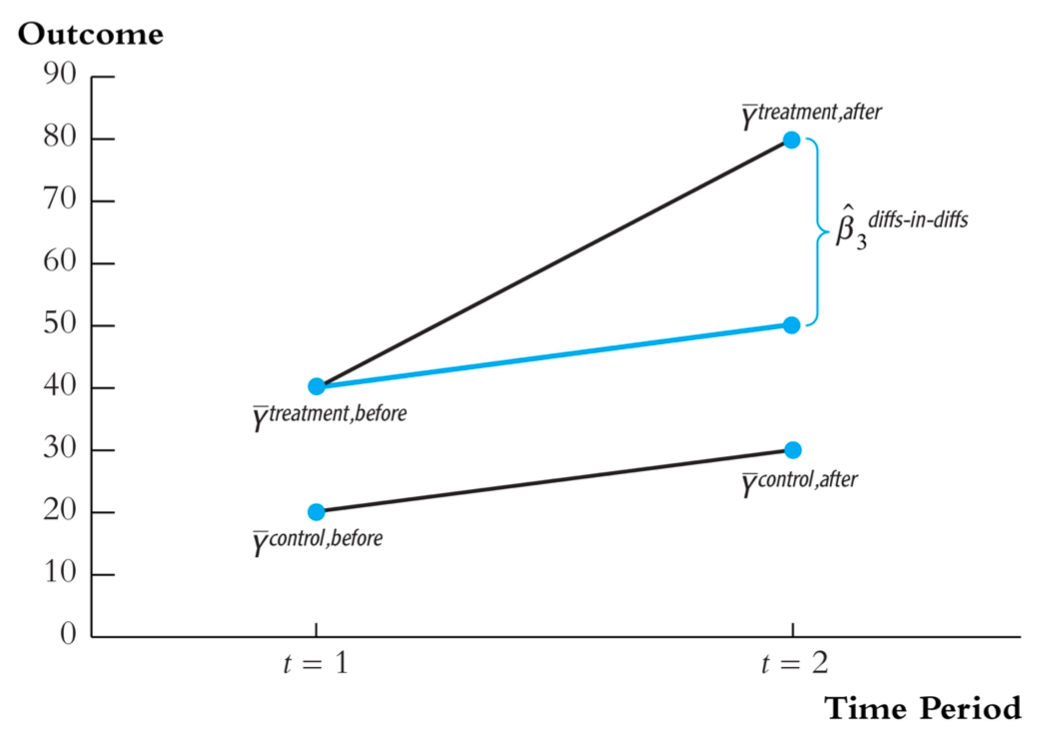
\includegraphics[width = \columnwidth]{Screen Shot 2023-05-25 at 14.18.58.png}

\subsection{DiD Regression}
$$Y=\beta_0 + \beta_1 post + \beta_2 treated + \beta_3 post \cdot treated + \epsilon$$
$post$ is a dummy variable, which is 1 after treatment

The post dummy controls for differences between the post-treatment
and pre-treatment period that do not differ between the treated and non-treated units (e.g., common economic shocks)
\section{Regression Discontinuity Design}
RDD is another specific type of quasi-experimental design that falls under the broader umbrella of observational studies. 

RDD is used to estimate causal effects by exploiting a discontinuity in the assignment of treatment based on a specific threshold or cutoff point.

In RDD, participants are assigned to treatment or control groups based on their position relative to a predetermined threshold or cutoff point of a continuous variable. The treatment effect is then estimated by comparing the outcomes of individuals just above and just below the threshold, assuming that there are no systematic differences between these groups other than their position relative to the threshold.

RDD is particularly useful when the treatment assignment is determined by a known and well-defined rule based on the value of a continuous variable. This design allows researchers to identify a causal effect precisely at the threshold, where individuals on either side of the threshold are expected to be similar in all relevant aspects, except for the treatment status.

The key idea behind RDD is that, if the treatment effect changes sharply and discontinuously at the threshold, any observed differences in outcomes between the treatment and control groups can be attributed to the treatment itself rather than other confounding factors.

\subsection{RDD \& challenges in estimating causal effects}

\subsubsection{Endogeneity} RDD exploits the fact that treatment assignment is determined by a predetermined threshold rather than being based on unobserved characteristics. This helps mitigate endogeneity issues that arise when the treatment assignment is related to the outcome of interest.
\subsubsection{Selection Bias} RDD compares units on either side of the threshold, where the treatment status changes abruptly. By focusing on this sharp transition, RDD effectively isolates the treatment effect from selection bias that may arise due to systematic differences between treatment and control groups.
\subsubsection{OVB} RDD assumes that any unobserved variables that affect the outcome variable change smoothly and continuously around the threshold. This reduces the potential bias from omitted variables that do not change abruptly at the threshold.

\subsection{Sharp Design}
In sharp design: probability of treatment jumps from 0 to 1 at R*

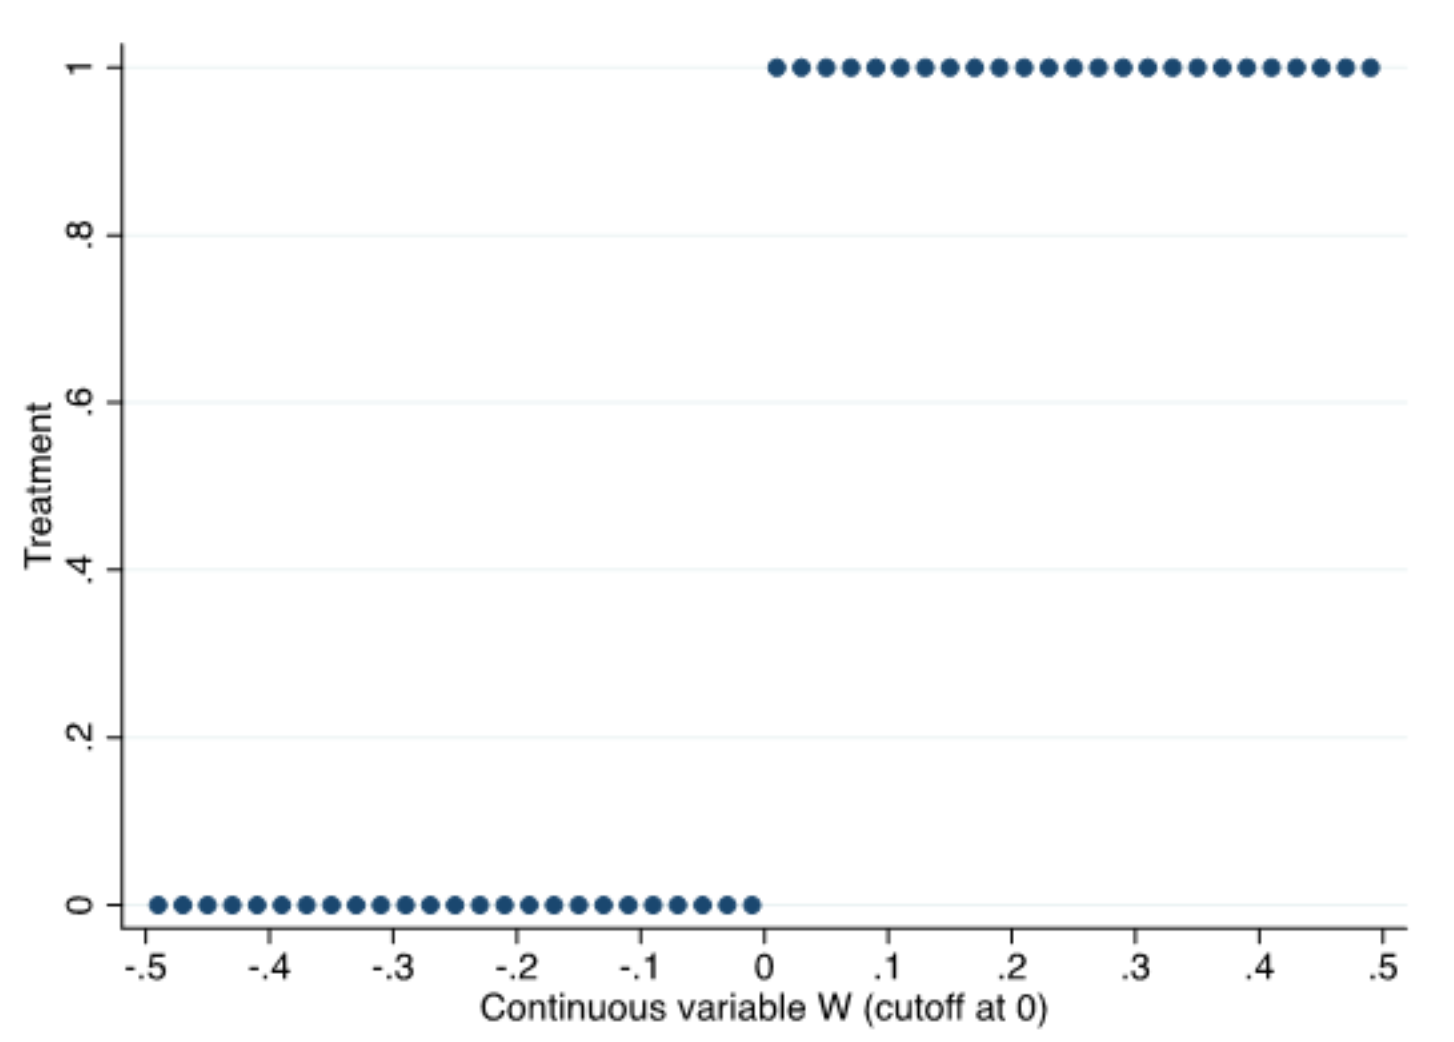
\includegraphics[width = \columnwidth]{Screen Shot 2023-05-30 at 14.30.35.png}

\subsection{Fuzzy Design}
In fuzzy design: probability of treatment increases discontinuously at R*

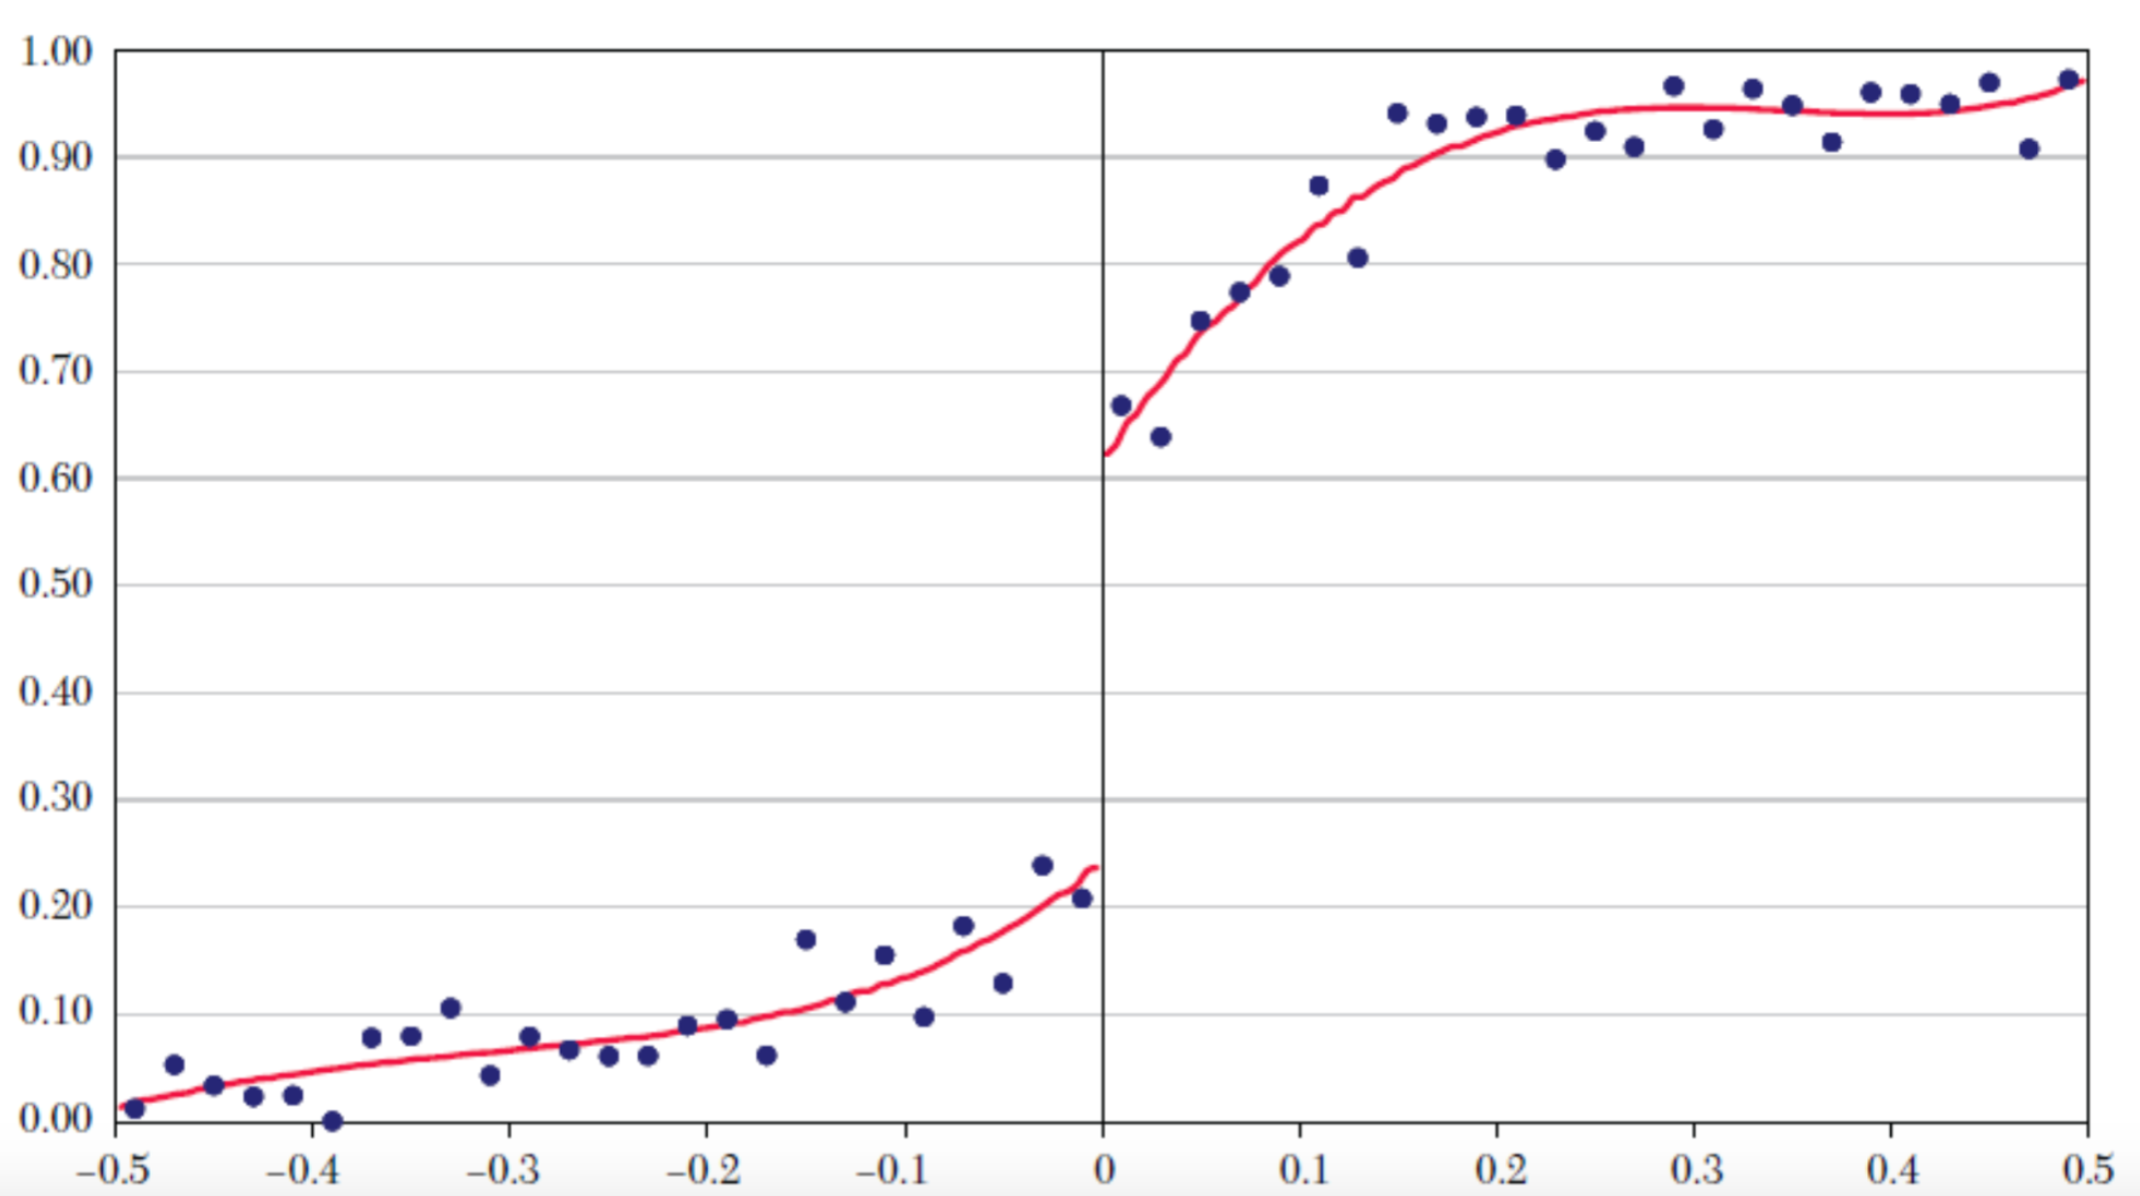
\includegraphics[width = \columnwidth]{Screen Shot 2023-05-30 at 14.31.58.png}

Treatment does not jump from 0 to 1 at the cutoff; some people get treatment below the cutoff and/or some don't get treatment above the cutoff

\subsection{Treatment Effect in RDD}
compare treated and non-treated entities, but only compare those who were barely treated (those with R slightly above R*) with those were barely not treated (those with R slighly below R*)
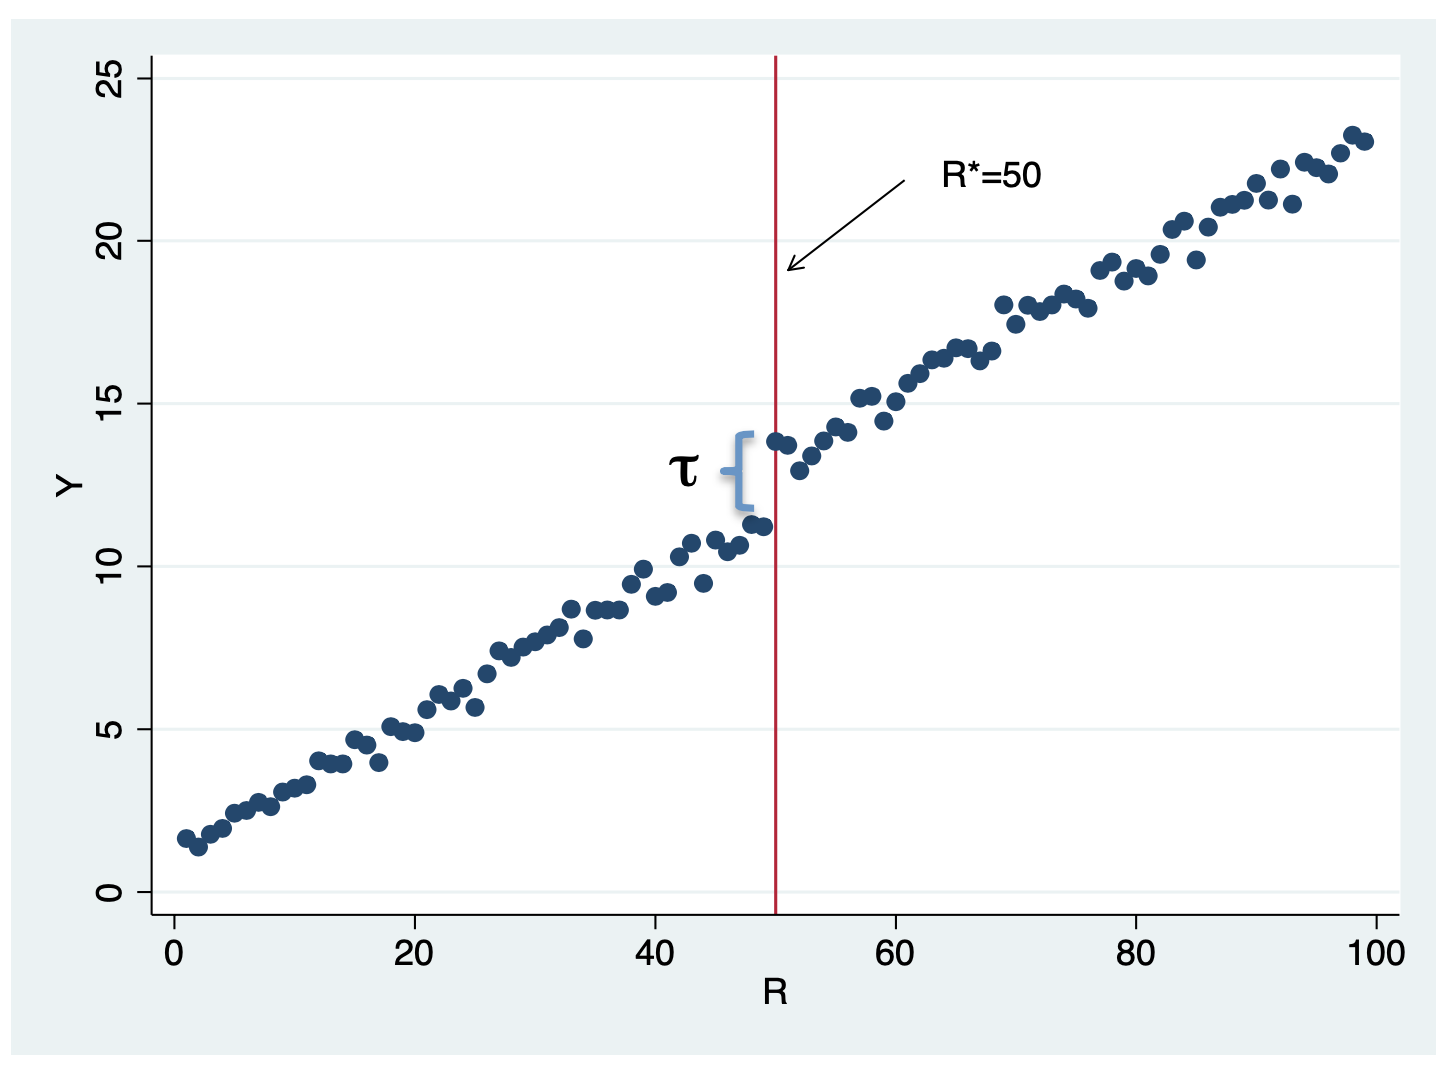
\includegraphics[width = \columnwidth]{Screen Shot 2023-05-30 at 15.12.59.png}

$$\tau=lim_{R \to R^{*+}}E(Y|R=R^*)-lim_{R \to R^{*-}}E(Y|R=R^*)$$

Using data near R*, estimate a regression with following independent variables:\begin{itemize}
    \item polynomial function of R (e.g., $R + R^3$)
    \item a dummy variable D which is equal to 1 if R$>$R* and 0 otherwise
    \item an interaction between D and the polynomial of R
\end{itemize}

For the linear case:
$$Y=\beta_0 + \beta_1 R + \beta_2 D + \beta_3 D \cdot R + \epsilon$$
$$\tau = \beta_2$$

Where $R$ is simply the running variable or a polynomial function of it. And $D$ a dummy that indicates if there was treatment or not.

$\beta_3 \ $ allows the slope of the relationship between R (called the running or forcing variable) and Y to be different after R*. This allows the relationship between R and Y to be flexible.

\paragraph{Reduced form relationship}
relationship between the outcome and treatment.

In the previous example the reduced-form regressions is $Y=\beta_0 + \beta_1 R + \beta_2 D + \beta_3 D \cdot R + \epsilon$. 

And the reduced form parameter: $\beta_2$

\paragraph{First stage regression}
$T= \pi_0 + \pi_1 R + \pi_2 D + \pi_3 D \cdot R + u $ where $T$ is Treatment. It estimates the relationship between the running variable and treatment assignment.

First-stage parameter: $\pi_2$

\subsection{Assumptions}
\begin{enumerate}
    \item Entities are Similar on Either Side of R*
    \item No Sorting around R*
    \item Continuity Assumption: The potential outcomes vary smoothly with the running variable (e.g., score) around the cutoff point. This assumption implies that there are no sudden jumps or discontinuities in the outcome variable at the cutoff, except for the treatment effect.
    \item No other policies at $R^*$/at the same time/cut-off
\end{enumerate}

%\section{Results from Methods}

%\begin{tabular}{l l}
%    OLS & ATE \\
 %   IV & LATE \\
  %  & ATE in case of effect homogeneity \\
   % DiD & ATT \\
%    FE & within-group treatment effect\\
 %   RDD & causal effect for  individuals close to cutoff \\
  %  Matching & ATE ATT \\&(ATC with inverse propensity score weighting)\\
%\end{tabular}

%By weighting the control group observations using inverse propensity scores, the analysis effectively creates a synthetic control group that resembles the treated group in terms of the observed covariates. This allows for estimating the Average Treatment Effect for the Control (ATC).

%FE + IV model can be augmented with an IV approach to estimate the ATE by leveraging both within-group and between-group variation.

%DiD + FE: Can estimate the average treatment effect (ATE) by comparing the treatment and control groups before and after the treatment. The FE controls for time-invariant unobserved heterogeneity, while the DiD design captures the differential treatment effect between the groups.

\newpage

\section{Other Useful Things}
\subsection{Computation of AT*}
$$ATE=\frac{ATC+ATT}{2}$$
$$ATC=(2\cdot ATE)-ATT$$
$$ATT=(2\cdot ATE)-ATC$$

\subsection{Statistical Significance (t-statistic)}
$$\frac{\beta_1}{SE}=t > 1.96 \Rightarrow \text{statist. significant}$$

or approximately: if $2 \times SE < \beta_1  \Rightarrow \text{statist. significant}$

\subsection{\hl{Log-Transformed Variables}}


\subsubsection{Only $Y$ transformed}
When the dependent variable is transformed using the ln function, the estimated coefficients can be interpreted as elasticities.

Linear change in the independent variable is associated with multiplicative change in the
dependent variable.
$$ln(Y)=B_0 + B_1\cdot X + u$$
A change in X by one unit ($\Delta X=1$) is associated with a \hl{$100 \times  (e^{B_1} - 1)  \ $} percent change in Y

$\approx$ A 1\% change in the independent variable is associated with a $B_1$ percentage change in the dependent variable.


\subsubsection{Only $X$ Transformed}
$$Y=B_0 + B_1 \cdot ln(X) + u$$ A 1\% change in X is associated with a \hl{change in Y of 
$B_1 \times ln(1.01) \approx 0.01 \times B_1$}

\subsubsection{Both $X, Y$ Transformed}
$$ln(Y)=B_0 + B_1 \cdot ln(X) + u$$
A 1\% change in X is associated with a $B_1\%$ change in Y, so $B_1$ is the elasticity of Y with respect to X.

Or a one-percent increase in $X$ is associated with a \hl{$100 \times (1.01^{B_1} - 1)$} percent change in $Y$

\section{Terminology}

\subsection{ \hl{Dependent variables} \ / $Y$}

\paragraph{/ Outcome of interest} the variable that is being predicted or explained by the independent variables in a regression model. 


\paragraph{Endogenous outcome of interest}  the outcome variable itself is affected by factors that are not directly accounted for in the regression model. In other words, the outcome variable is endogenous, meaning it is correlated with the error term or the unobserved factors.

The endogeneity of the outcome variable can arise due to feedback loops, reverse causality, omitted variable bias, or other factors. These feedback relationships can create a bidirectional relationship, where changes in the outcome variable can simultaneously affect the independent variables, introducing endogeneity issues.

\subsection{\hl{Independent variables} \ / $X_n$}  
\paragraph{explanatory variable/ predictor variable/ regressor} is a variable used to explain or predict the variation in the outcome variable. It is the variable that is believed to have a causal or explanatory relationship with the outcome variable.

\paragraph{Statistical independence} also orthogonality, refers to the lack of correlation or association between two variables. If two variables are statistically independent, knowing the value of one variable provides no information about the value of the other variable.


\paragraph{Endogeneous regressor} independent variables in a regression model that are correlated with the error term. Endogeneity arises when there is a feedback relationship between the independent variables and the error term, leading to biased and inconsistent estimates.

\paragraph{Predicted endogenous explanatory variable} This refers to the estimated or predicted values of an endogenous explanatory variable in a regression model. These predicted values are obtained using instrumental variable techniques or other methods to address endogeneity.

\subsection{Endo-/Exogeneity}


\subsubsection{\hl{Exogeneity}}
 refers to the absence of a direct causal relationship between a variable and the error term.

Changes in the exogenous variable are not caused by or do not cause changes in the other variables in the model. It also does not influence unobserved factors that affect the dependent variable, in other words is not correlated with the error term.

\subsubsection{\hl{Endogeneity}} refers to a situation in which a variable of interest is correlated with the error term.

This correlation implies that there is a systematic relationship between the independent variable and the unobserved factors that affect the dependent variable.

To provide some intuition, let's consider an example. Suppose you are studying the relationship between education (independent variable) and income (dependent variable). If education is endogenous, it means that there are unobserved factors, such as innate ability or motivation, that affect both education and income.

\hl{Endogeneity can arise due to} 

\paragraph{Omitted Variables} If relevant explanatory variables are omitted from the model, and these omitted variables are correlated with both the included variables and the error term, endogeneity occurs.

\paragraph{Measurement Error} If there are errors in the measurement of the variables, it can introduce endogeneity. Measurement errors that are correlated with the error term can lead to biased estimates.

\paragraph{Sample Selection Bias} Endogeneity can arise in cases of sample selection bias, where the sample used for analysis is not representative of the population of interest. The selection process can be related to the outcome variable and the explanatory variables, resulting in endogeneity.

\paragraph{Reverse Causality} /endogeneous selection/ refers to a situation in which the  presumed cause and effect relationship between two variables is reversed or runs in the opposite direction of what is initially assumed. In other words, the outcome variable is causing changes in the explanatory variable(s), rather than the other way around.

\paragraph{bidirectional causality / feedback loop}  the idea that the causal relationship between variables operates in both directions. Changes in one variable can influence the other variable, and vice versa.

\paragraph{Endogeneous determination} This term highlights that the determination of the variables is influenced by internal factors within the system, rather than being solely driven by external factors.

\paragraph{Simultaneity}
 refers to a situation where the relationship between two variables is bidirectional and occurs simultaneously. In other words, both variables are not only influencing each other but are also being influenced by each other at the same time.
 
\subsection{Challenges when establishing Causal Effects}

Estimating causal effects poses several challenges that need to be carefully addressed to obtain valid and reliable results. Some of the key challenges include:

\paragraph{Endogeneity} Endogeneity occurs when the independent variable is correlated with the error term in the regression model, leading to biased and inconsistent estimates. Addressing endogeneity requires the use of appropriate techniques such as instrumental variable (IV) estimation or natural experiments.

$\Rightarrow$ IV

\paragraph{Confounding} Confounding arises when there are unobserved factors that affect both the independent variable and the dependent variable. These confounders can distort the estimated causal relationship. Techniques such as matching, propensity score matching, or regression adjustment can be used to control for confounding variables.

$\Rightarrow$ Matching

For time-varying confounders $\Rightarrow$ DiD

\paragraph{Selection Bias} Selection bias occurs when the sample used for analysis is not representative of the target population, leading to biased estimates. To mitigate selection bias, techniques such as random sampling, propensity score matching, or difference-in-differences (DiD) analysis can be employed.

\paragraph{Measurement Error} Measurement error in the variables used in the analysis can introduce bias and imprecision in the estimated causal effects. Proper measurement techniques, validation, and sensitivity analysis can help mitigate measurement error issues.

\paragraph{Noncompliance and Treatment Spillover} In experiments or interventions where individuals may not comply with the assigned treatment or where the treatment may spill over to non-treated individuals, the estimated causal effects may be affected. Techniques such as instrumental variable analysis or intention-to-treat analysis can address noncompliance and treatment spillover issues.
Sample Size and Statistical Power: Inadequate sample size can limit the ability to detect and estimate small causal effects accurately. Large sample sizes are generally required to obtain precise and reliable estimates. Power calculations can help determine the required sample size for detecting specific effect sizes.

\paragraph{External Validity} Estimating causal effects within a specific study sample may not necessarily generalize to the broader population or other contexts. Assessing the external validity of the estimated effects is important to understand the applicability and generalizability of the findings.

\subsection{Other Terms}
\subsubsection{Unobserved determinants} These are unobserved factors or variables that influence the outcome variable but are not directly measured in the data. They can introduce bias if they are correlated with both the independent variables and the error term.

\subsubsection{Residual/error term} This represents the unexplained variation in the dependent variable that is not accounted for by the independent variables.

\subsubsection{Multicollinearity} occurs when there is a high correlation between two or more independent variables in a regression model. It can cause problems in estimation and interpretation of the regression coefficients.

\subsubsection{Heteroskedasticity} Heteroskedasticity refers to the situation where the variability of the error term is not constant across different values of the independent variables. It violates one of the assumptions of classical linear regression, leading to inefficient and inconsistent estimates.

\subsubsection{Autocorrelation} also known as serial correlation, refers to the correlation between error terms in a time series or panel data regression model. It violates the assumption of independence of errors and can lead to biased and inefficient parameter estimates.

\subsubsection{Simultaneity} Simultaneity refers to a situation where two or more variables are jointly determined and affect each other simultaneously. It poses challenges in estimating the causal relationship between the variables and requires special econometric techniques to address.

\subsubsection{Observables}
observables refer to variables or factors that can be directly measured or observed in a study or dataset.

\subsubsection{latent variable} /hidden variable/unobserved variable, is a construct that is not directly measured or observed but is inferred from observed indicators or measurements.

\subsubsection{Controll variables $\equiv$ covariates}

\subsubsection{Interactions}
interactions refer to the combined effect of two or more variables on an outcome or response variable. An interaction occurs when the relationship between two or more variables is not simply additive or independent, but rather influences the outcome in a way that is dependent on the values of the interacting variables.

Interactions can be expressed in statistical models using interaction terms, which are created by multiplying the values of two or more variables together.

\subsubsection{Effect heterogeneity}
Effect heterogeneity refers to the variation in treatment effects across different individuals or groups.

\subsubsection{$R^2$}
provides an indication of how well a regression model fits the observed data. It quantifies the proportion of the variance in the dependent variable that is explained by the independent variables in the model.

ranges from 0 to 1. An R-squared value of 0 means that the regression model explains none of the variation in the dependent variable, while an R-squared value of 1 means that the model explains all the variation.

R-squared $(R^2)$ is calculated as the proportion of the explained sum of squares (ESS) divided by the total sum of squares (TSS). Here's the formula:

$$R^2 = ESS / TSS$$

\paragraph{Explained sum of squares (ESS)} represents the sum of the squared differences between the predicted values of the dependent variable and the mean of the dependent variable. It captures the variability in the dependent variable that is explained by the independent variables in the regression model.
$$ESS = \Sigma(\hat{y} - \Bar{y})^2$$

\paragraph{Total sum of squares (TSS)} represents the sum of the squared differences between the actual values of the dependent variable and the mean of the dependent variable. It represents the total variability in the dependent variable.
$$ESS = \Sigma(y - \Bar{y})^2$$
\subsubsection{f-test}
Tests if several independent variables are jointly significant.

\subsubsection{t-test}
t-test is a statistical test used to determine whether there is a significant difference between the means of two groups or conditions. It is based on the t-distribution and is commonly used in hypothesis testing.

\subsubsection{restriction}

\subsubsection{Identifying assumption}
When one is interested in establishing causal effect, a condition imposed on the model that allows for causal interpretation of the estimate is called an identification assumption.



\end{multicols*}
\end{document}